
% =========================================================================== %
\chapter{Preliminaries}
\label{chap:prelim}
% =========================================================================== %



  Permutations are a fundamental mathematical concept used productively
  throughout the sciences to encode and understand disorder and rearrangement. 
  The theory of permutation patterns captures this geometric notion of
  disorder, and has yielded a wide variety of productive and surprising
  research over the past several decades. This dissertation presents several
  interrelated projects within this interesting and rapidly developing field.
  Structural, analytic, and probabilistic combinatorics are central to this
  work, and combine to provide unique insight into pattern enumeration. 

  This dissertation is organized as follows: Chapter~\ref{chap:prelim} provides
  an accessible introduction to the ideas and methods at play, followed by four 
  illustrative examples which serve to motivate and introduce the material
  to come. The following four chapters represent self-contained projects
  utilizing these techniques.  Each of these chapters is based partly on
  separate publications~\cite{me-expat,me-polyclass,me-fixpat,me-involutions},
  but together they speak to the utility of structural methods coupled with
  multivariate analysis.  Recursive structural decomposition intersected with
  modern analytic and probabilistic techniques has proven exceptionally useful
  in investigating patterns within permutations, and each chapter focuses on a
  separate facet of this productive combination. 
  
  For an accessible introduction to the field of combinatorics, the reader is
  directed to B\'ona~\cite{BonaWalk}. Stanley~\cite{Stanley1, Stanley2}
  provides a more advanced treatment to the subject as a whole, while
  B\'ona~\cite{BonaPerm} focuses on the combinatorics of permutations. 
  Wilf~\cite{wilfbook} gives an excellent introduction to the theory of
  generating functions, while Petkov\v{s}ek, Wilf, and Zeilberger~\cite{A=B}
  provide a survey of algorithmic methods. 
  Finally, analytic methods in combinatorics are presented best by Flajolet and
  Sedgewick~\cite{flajolet} and by Pemantle and Wilson~\cite{pemantle}, who
  focus on single- and multi-variate methods, respectively.


% =========================================================================== %
\section{Permutation Classes}
\label{prelim:sec:perms}
% =========================================================================== %

  \index{permutation}
  Permutations owe much of their rich structure to their variety of equivalent
  representations.  In this section we establish some of the basic notation and
  definitions of permutations and permutation classes. Throughout this
  dissertation, let $\Zgeq$ denote the non-negative integers $\{0, 1, 2, 3,
  \dots \}$, $\Pos$ the positive integers $\{1, 2, 3, 4, \dots\}$, and, for a given
  integer $n \in \Pos$, let $[n]$ denote the integers $\{1, 2, \dots n\}$. 

  \subsection{Permutations and Patterns}


    \begin{definition}\label{prelim:def:perm}
      For a given integer $n \in \Pos$, a \emph{permutation of length $n$}
      is a sequence $\pi = \pi_1 \pi_2 \dots \pi_n$ in which
      $\pi_i \in [n]$ and each integer of $[n]$ is used exactly once. There are
      $n!$ permutations of length $n$, the set of all of which is denoted $\S_n$. 
    \end{definition}

    
    For example, the six permutations of length three are as follows: 
    $$ \S_3 = \{123, 132, 213, 231, 312, 321\}. $$

    Permutations can be represented in many different ways, each leading to
    different generalizations. The above definition is known as the
    \emph{one-line representation} in the literature, and this approach leads
    naturally to the theory of permutation patterns. We start by presenting
    formal definitions of patterns before providing a geometric motivation. 


    \begin{definition} \label{prelim:def:orderiso}
      For a positive integer $n$ any two sequences of distinct numbers $\alpha
      = \alpha_1 \alpha_2 \dots \alpha_n$ and $\beta = \bta_1 \bta_2 \dots
      \bta_n$, we say that $\alpha$ and $\bta$ are \emph{order isomorphic}
      (denoted $\alpha \sim \bta$) if
      $$ \alpha_i < \alpha_j \quad \text{if and only if} 
          \quad \bta_i < \bta_j.$$
    \end{definition}

    For example, the sequences $\alp = 9\ 2\ 4$ is order isomorphic to $\bta  = 5\
    1\ 3$, because their entries share the same relative order: the first is
    the biggest, the second is smallest, and the third lies in between. 

    It follows that each sequence $\alpha$ of $n$ distinct numbers is order
    isomorphic to a unique permutation of length $n$, called the \emph{standardization}
    of $\alpha$, and  denoted $\std(\alpha)$. For a given sequence $\alpha$, the
    standardization can be constructed by relabelling the smallest entry of of
    $\alpha$ by $1$, the second smallest by $2$, and so on (i.e., $\std(9\ 2\
    4) = 3\ 1\ 2$). We can now present the formal definition of permutation
    patterns. 

    \begin{definition} \label{prelim:def:patterns}
      Let $n, k \in \Pos$ with $k \leq n$, and let $\pi = \pi_1 \pi_2 \dots
      \pi_n \in \S_n$ and $\sg = \sg_1 \sg_2 \dots \sg_k \in
      \S_k$. Say that $\sg$ is \emph{contained as a pattern} in $\pi$ (denoted
      $\sg \prec \pi$) if there is some subsequence $1 \leq i_1 < i_2 < \dots
      <i_k \leq n$ such that 
      $$ \pi_{i_1} \pi_{i_2} \dots \pi_{i_k} \sim \sg_1 \sg_2 \dots \sg_k.$$
    \end{definition}


    Note that pattern containment is \emph{reflexive}
    ($\pi \prec \pi$ for all permutations $\pi$), \emph{transitive} ($\ro \prec
    \sg$, $\sg \prec \pi$ implies $\ro \prec \pi$), and \emph{anti-symmetric}
    ($\sg \prec \pi$ and $\pi \prec \sg$ implies $\sg = \pi$). These three
    properties mean that the set of all permutations, equipped with this
    ordering, forms a partially ordered set (a poset) known as the
    \emph{pattern poset}. 
    

    \begin{figure}[t] \centering
      \scalebox{1}{
        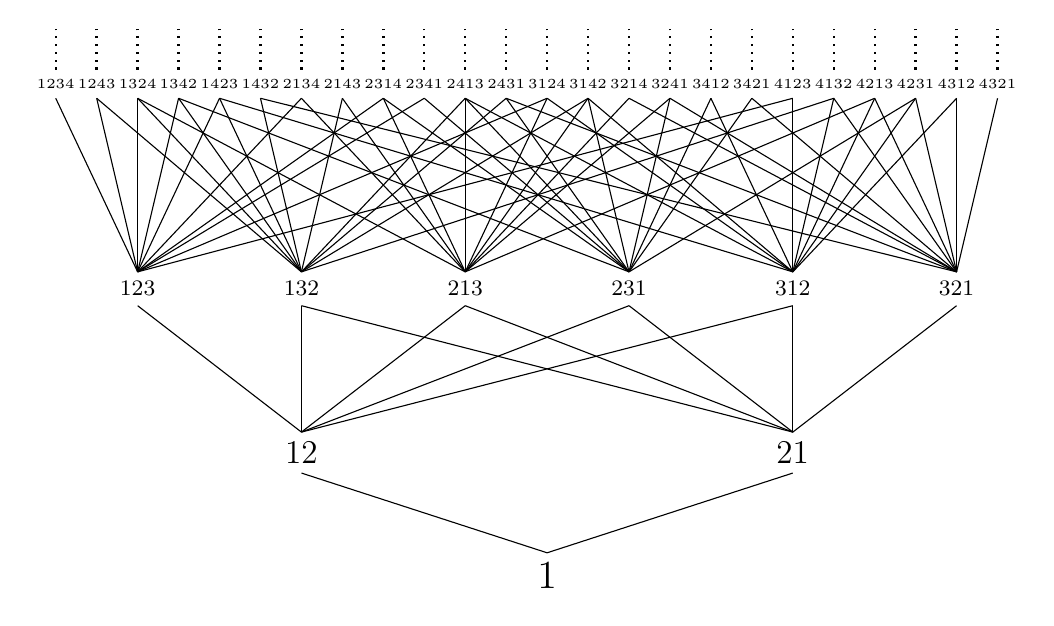
\begin{tikzpicture}[
        every node/.style={},
         scale=.52]
          \node (1) at (12,0) {\Large 1};

          \node (12) at (6,3)  {\large 12};
          \node (21) at (18,3) {\large 21};

          \draw (12.south)-- (1.north);
          \draw (21.south) -- (1.north);

          \node (123) at (2 ,7) {\footnotesize 123};
          \node (132) at (6 ,7) {\footnotesize 132};
          \node (213) at (10,7) {\footnotesize 213};
          \node (231) at (14,7) {\footnotesize 231};
          \node (312) at (18,7) {\footnotesize 312};
          \node (321) at (22,7) {\footnotesize 321};

          \draw (123.south) -- (12.north);
          \draw (132.south) -- (12.north);
          \draw (213.south) -- (12.north);
          \draw (231.south) -- (12.north);
          \draw (312.south) -- (12.north);
          
          \draw (132.south) -- (21.north);
          \draw (213.south) -- (21.north);
          \draw (231.south) -- (21.north);
          \draw (312.south) -- (21.north);
          \draw (321.south) -- (21.north);
          
          \node (1234) at (0 ,12) {\tiny 1234};
          \node (1243) at (1 ,12) {\tiny 1243};
          \node (1324) at (2 ,12) {\tiny 1324};
          \node (1342) at (3 ,12) {\tiny 1342};
          \node (1423) at (4 ,12) {\tiny 1423};
          \node (1432) at (5 ,12) {\tiny 1432};

          \node (2134) at (6 ,12) {\tiny 2134};
          \node (2143) at (7 ,12) {\tiny 2143};
          \node (2314) at (8 ,12) {\tiny 2314};
          \node (2341) at (9 ,12) {\tiny 2341};
          \node (2413) at (10,12) {\tiny 2413};
          \node (2431) at (11,12) {\tiny 2431};

          \node (3124) at (12,12) {\tiny 3124};
          \node (3142) at (13,12) {\tiny 3142};
          \node (3214) at (14,12) {\tiny 3214};
          \node (3241) at (15,12) {\tiny 3241};
          \node (3412) at (16,12) {\tiny 3412};
          \node (3421) at (17,12) {\tiny 3421};

          \node (4123) at (18,12) {\tiny 4123};
          \node (4132) at (19,12) {\tiny 4132};
          \node (4213) at (20,12) {\tiny 4213};
          \node (4231) at (21,12) {\tiny 4231};
          \node (4312) at (22,12) {\tiny 4312};
          \node (4321) at (23,12) {\tiny 4321};

          % 123
          \foreach \p in {1234, 1243, 1324, 1342, 1423, 2134, 2314, 2341, 3124, 4123}
            \draw (\p.south) -- (123.north);
          % 132
          \foreach \p in {1243, 1324, 1342, 1423, 1432, 2143, 2413, 2431, 3142, 4132}
            \draw (\p.south) -- (132.north);
          % 213
          \foreach \p in {1324, 2134, 2143, 2314, 2413, 3124, 3142, 3214, 3241, 4213}
            \draw (\p.south) -- (213.north);
          % 231
          \foreach \p in {1342, 2314, 2341, 2413, 2431, 3142, 3241, 3412, 3421, 4231}
            \draw (\p.south) -- (231.north);
          % 312
          \foreach \p in {1423, 2413, 3124, 3142, 3412, 4123, 4132, 4213, 4231, 4312}
            \draw (\p.south) -- (312.north);
          % 321
          \foreach \p in {4321, 3421, 4231, 2431, 3241, 4312, 4132, 1432, 4213, 3214}
            \draw (\p.south) -- (321.north);

          \foreach \p in {1234, 1243, 1324, 1342, 1423, 1432,
                          2134, 2143, 2314, 2341, 2413, 2431,
                          3124, 3142, 3214, 3241, 3412, 3421,
                          4123, 4132, 4213, 4231, 4312, 4321}
            \draw[dotted, line width=.3mm] (\p.north) -- ++(0,1);
        \end{tikzpicture}
        }
    \caption[The first four levels of the permutation pattern poset.]{
          The first four levels of the permutation pattern poset. Two
          permutations are connected by a line if one is contained in the other
          as a pattern.}
    \label{prelim:fig:poset}
    \end{figure}

    The first four levels of this poset are shown in
    Figure~\ref{prelim:fig:poset}. Note that the number of lines going up from
    each permutation depends only on the length of the permutation, while the
    number going down varies. This will be a topic of study in
    Chapter~\ref{chap:fixpat}, where we will establish the probability
    distribution for the number of large patterns contained within randomly
    selected permutations. 

    If a permutation $\pi$ does not contain a pattern $\sg$, we say that $\pi$
    \emph{avoids} $\sg$. The set of all permutations which avoid a fixed
    pattern $\sg$ is denoted $\Av(\sg)$. Transitivity of pattern containment
    implies that if $\pi \in \Av(\sg)$ and $\ro \prec \pi$, then $\ro \in
    \Av(\sg)$. This relationship motivates our next definition. 



    \begin{definition}\label{prelim:def:class}
      Let $\cP$ be a poset. A subset $S \subseteq \cP$ is called a
      \emph{downset} if it is closed downwards. That is, if $x \in S$ and $y
      \prec x$, then $y \in S$. 
      A downset of the permutation pattern poset is called a \emph{permutation
      class}. For a permutation class $\C$, denote by $\C_n$ the set of
      permutations of length $n$ in $\C$. 
    \end{definition}


    The set of all patterns which avoid some specified set of patterns are
    known as the \emph{avoidance classes}, and were first introduced by
    Knuth~\cite{Knuth} in the context of stack sorting.  The investigation of
    these and other classes has sparked a wide range of research over the past
    several decades, with a focus on enumeration.  In
    particular, the question of `which pattern is easiest to avoid?' has been a
    major open question for many years, and a variety of techniques have been
    developed to provide partial answers. The Marcus-Tardos
    Theorem~\cite{MarcusTardos} (which stood open as the Stanley-Wilf
    Conjecture for two decades) motivates much of this work.

    \begin{definition} \label{prelim:def:growthrate}
      Let $\C$ be a permutation class. The \emph{(upper) growth rate} of $\C$ is
      defined as the limit
      $$ \limsup_{n \ra \infty} \sqrt[n]{|\C_n|}.$$
    \end{definition}

    \begin{theorem}[Marcus, Tardos~\cite{MarcusTardos}] \label{thm:MarcusTardos}
      Every proper permutation class has a finite growth rate. 
    \end{theorem}



  \subsection{Wilf-Equivalence}
    
    Though Theorem~\ref{thm:MarcusTardos} says that all proper permutation classes
    have a finite growth rate, finding and classifying these growth
    rates is difficult. Of particular interest is identifying
    those patterns which have the same enumeration, i.e., $\bta, \tau$ such
    that $\Av_n(\bta) = \Av_n(\tau)$ for all $n$. Such a pair $\bta, \tau$ are
    called \emph{Wilf-equivalent}, and the set of all Wilf-equivalent
    permutations form a \emph{Wilf class}. Though showing Wilf-equivalence can be
    hard in general, many equivalences arise from eight trivial symmetries. 

    \begin{definition} \label{prelim:def:symmetries}
      Let $\pi = \pi_1 \pi_2 \dots \pi_n$ a permutation. The
      \emph{reverse}, the \emph{complement}, and the \emph{inverse} of $\pi$
      (denoted $\pi^r$, $\pi^c$, and $\pi^{-1}$, respectively) are defined as
      follows:
      $$ \begin{aligned}
        \left(\pi^r\right)_i &= \pi_{n-i + 1}, \\
        \left(\pi^c\right)_i &= n - \pi_{i} + 1, \text{ and } \\
        \left(\pi^{-1}\right)_{\pi_i} &= i. \\
      \end{aligned} $$
    \end{definition}
    
    Each of these operations map the set of permutations to itself, and each
    \emph{preserves pattern containment}. That is, if $\sg \prec \pi$, then
    $\sg^i \prec \pi^i$, for each $i \in \{r, c, -1\}$. It follows than that
    the class of permutations avoiding a pattern are in bijection with the
    class avoiding any symmetry of this pattern. These three symmetries
    thus generate an automorphism group of the pattern poset, which is
    isomorphic to the dihedral group of order eight. Of these three, only the
    inversion map has any fixed points; a permutation which is its own inverse
    is called an \emph{involution}.  It follows from Smith~\cite{Smith2006}
    that this is the complete set of automorphisms which respect pattern
    containment. Note that further order-respecting isomorphisms between classes
    are explored in Albert, Atkinson and Claesson~\cite{Claesson2013}. Note
    further that Wilf-classes need not contain bases of the same size: 
    Burstein and Pantone~\cite{pantone2014} recently showed the
    Wilf-equivalence of $\Av(1324, 3416725)$ and 
    $\Av(2143,3142,246135)$. 

    For permutations of length three, $123$ and $321$ are complements (and
    reverses) of each other, and thus the classes $\Av(123)$ and $\Av(321)$ 
    have the same enumeration (i.e., $|\Av_n(123)| = |\Av_n(321)|$ for all $n
    \in \Zgeq$). The permutation $132$ can be reversed to obtain $231$ or
    complemented to obtain $312$, and $312$ can be complemented to obtain
    $213$. Therefore the permutations $\{132, 213, 231, 312\}$ are
    Wilf-equivalent, and so there are at most two Wilf classes for length $3$
    permutations. 

    MacMahon, in 1915/16~\cite{PercyBook} enumerated the $123$-avoiding
    permutations while Knuth, in 1968~\cite{Knuth}, enumerated the
    $231$-avoiding permutations, leading to the first non-trivial Wilf
    equivalence. A bijection between $123-$ and $132$-avoiding permutations was
    presented by Simion and Schmidt~\cite{Simion1985} in 1985.

    \begin{theorem}[MacMahon, Knuth~\cite{PercyBook, Knuth}]
    \label{prelim:thm:knuth-equiv}
      The number of permutations of length $n$ avoiding $123$ is equal to the number
      avoiding $231$. 
    \end{theorem}

    We explore this result further in Sections~\ref{prelim:sec:av132}
    and~\ref{prelim:sec:av123}, and rederive this result using geometric
    constructions. Note that two Wilf-equivalent classes can have sharply
    contrasting structure, as we will soon see is the case for $\Av(123)$ and
    $\Av(132)$. 
    Theorem~\ref{prelim:thm:knuth-equiv} shows that there is only one Wilf
    class for length three patterns, which gives false hope for longer
    patterns.
    As we see here, the situation becomes much more complicated as patterns get
    longer. 

    Of the twenty-four patterns of length four, the trivial symmetries show
    that there are at most eight Wilf classes. 
    Non-trivial theorems from Babson and West~\cite{BabsonWest} and
    West~\cite{WestDiss} (and generalized in Backelin, West, and
    Xin~\cite{Backelin2007}) reduce this number to four, and 
    a result of Stankova~\cite{Stankova1994} shows that two of these
    remaining classes are Wilf-equivalent. This leaves the patterns of length
    four partitioned into three Wilf classes. That these three classes do in
    fact have different enumerations can be seen in the data presented in
    Table~\ref{prelim:tab:four-classes}. 

    \begin{table}[t] \centering
      \caption{Enumerations of the three Wilf classes for patterns of length
      four.}
      \label{prelim:tab:four-classes}
      \begin{tabular}{rrrrrrrrr}
      \multicolumn{9}{c}{$|\Av_n(\bta)|$} \\ 
       $n = $ & 1  & 2 & 3 & 4  & 5 & 6 & 7 & 8
        \\ \hline
      $\bta = 1342$ &
        1 & 2 & 6 & 23 & 103 & 512 & 2740 & 15485 \\
      $\bta = 1234$ &
        1 & 2 & 6 & 23 & 103 & 513 & 2761 & 15767 \\
      $\bta = 1324$ &
        1 & 2 & 6 & 23 & 103 & 513 & 2762 & 15793 \\
      \end{tabular}
    \end{table}

    Note that the monotone pattern is neither the easiest nor hardest to avoid,
    as one might expect.  These three cases speak to the complexity involved in
    enumerating permutation classes. The class $\Av(1342)$ was first counted by
    B\'ona~\cite{Bona1997}, and was found to have an algebraic generating
    function and an exponential growth rate  of $8$. The class $\Av(1234)$ was
    enumerated by Gessel~\cite{Gessel1990} and Regev~\cite{Regev}, who provided
    an exact formula the number of permutations of a given length in the class
    and showed that the exponential growth rate is $9$, but showed that the
    generating function is D-finite but nonalgebraic. Finally, the class
    $\Av(1324)$ has not been enumerated and the growth rate is unknown, except
    that it is between $9.42$ (Albert et.  al.~\cite{1324LowerBound}) and
    $13.93$ (B\'ona~\cite{1324UpperBound}). 

    The permutation $1324$ is a \emph{layered} permutation, meaning it can be
    written as a sequence of decreasing runs, the entries of which are each
    larger than the previous layer. Layered permutations were conjectured by
    Arratia~\cite{Arratia1999} to be the easiest to avoid, i.e., their
    avoidance classes have the fastest growth. This conjecture led to interest
    in these patterns~\cite{Claesson2012, Bona2007, Elder2005}, but was
    recently overturned by Fox~\cite{Fox}, who showed that the situation is
    much more complex than small examples suggest. 
    In Chapter~\ref{chap:involutions}
    we consider the problem of finding growth rates of pattern avoiding
    \emph{involutions}, and determine the growth rates of two such sets
    avoiding patterns of length four. 
    


 

  \subsection{Geometric Motivation}
    
    The investigation and classification of Wilf classes is a deep and complex
    research program.  The primary focus of this dissertation, however, is on
    the \emph{geometric structure} of permutation classes, and the use of this
    structure to understand and explore pattern containment. The concepts
    presented above can all be reconsidered in a geometric context which allows
    for a more intuitive description of permutations
    and their patterns and symmetries. This geometric approach helps to
    illuminate new directions of research, is central to this work. 


    \begin{definition} \label{prelim:def:permplot}
      The \emph{plot} of the permutation $\pi$ of length $n$ is
      the set of points $(i, \pi_i) \in \bR^2$ for each $i \in [n]$. 
    \end{definition}

    \begin{figure}[t]\centering 
      \begin{tikzpicture}
        [scale = .3, line width = .5pt]

        \draw (0,12) -- (0,0) -- (12,0);
        \foreach \num in {2, 4,..., 10}
        {
          \draw (\num, 0) -- (\num, -.3);
          \draw (0, \num) -- (-.3, \num);
        }
        \foreach \y [count = \x] in {2,5,1,4,3}
          \draw[fill = black] (2*\x,2*\y) circle (2mm);
      \end{tikzpicture}
      \caption{The plot of the permutation $\pi = 2\ 5\ 1\ 4\ 3$.}
      \label{prelim:fig:plot}
    \end{figure}

    The plot of a permutation is shown in Figure~\ref{prelim:fig:plot}. 
    Say that a set of $n$ points in $\bR^2$ is \emph{generic} if no two points
    lie on the same horizontal or vertical line. 
    Say that two generic sets $P$ and $T$ are \emph{order isomorphic} (written
    $P \sim T$) if the axes can be stretched or shrunk in some way to transform
    one into the other. 
    
    It follows that every generic point set is order isomorphic to
    a unique permutation plot, and that order isomorphism is an equivalence
    relation.
    The set of all $n$-element generic point sets, modulo this relation, is
    therefore in bijection with the set of all permutations of length $n$. This
    correspondence allows us to identify a permutation with its plot, and
    provides an alternate geometric definition of permutation patterns,
    illustrated in Figure~\ref{prelim:fig:plotpattern}.

    \begin{definition} 
      Let $n,k \in \Pos$ with $k \leq n$, and let $\pi \in \S_n$ and $\sg \in
      \S_k$. Let $P, T$ be the points in the plots of $\pi$ and $\sg$,
      respectively. Say that $\sg \prec \pi$ if there is some subset $R
      \subseteq S$ for which $R \sim T$. 
    \end{definition}


    \begin{figure}[t]
      \centering
      \begin{tikzpicture}[scale = .4,
                          every node/.style={circle, fill=black, inner sep=.5mm},
                          greyed/.style={fill=lightgray}]
        \node at (2,5) {};
        \node at (3,1) {};
        \node at (5,3) {};
      \end{tikzpicture}
        \hspace{1pc}
        \raisebox{2pc}{$\subset$}
        \hspace{1pc}
      \begin{tikzpicture}[scale = .4,
                          every node/.style={circle, fill=black, inner sep=.5mm},
                          greyed/.style={fill=lightgray}]
        \node[greyed] at (1,2) {};
        \node[] at (2,5) {};
        \node at (3,1) {};
        \node[greyed] at (4,4) {};
        \node at (5,3) {};
      \end{tikzpicture}
        \hspace{1pc}
        \raisebox{2pc}{$= $}
        \hspace{1pc}
      \begin{tikzpicture}[scale = .4,
                          every node/.style={circle, fill=black, inner sep=.5mm},
                          greyed/.style={fill=gray}]
        \foreach \y [count = \x] in {2,5,1,4,3}
        \node at (\x,\y) {};
      \end{tikzpicture}

      \caption{The permutation $\sg = 312$ is contained in the permutation $\pi =
                25143$. }
      \label{prelim:fig:plotpattern}
    \end{figure}

    
    Many operations on permutations are easier to understand
    through these geometric plots. For example, the plot of a permutation can
    be reflected and rotated to produce new permutations. Letting $\pi = \pi_1
    \pi_2 \dots \pi_n$ be a permutation, the reverse of $\pi$ is obtained by
    reflecting the dots across a vertical line, the complement by reflecting
    across a horizontal line, and the inverse is obtained by reflecting across
    the line $y = x$. That these operations generate a group of automorphisms
    isomorphic to the dihedral group of order eight is clear when
    viewing permutations as plots within a square. It is equally clear from
    this viewpoint that these operations respect pattern containment
    
    
    We can also define operations which act on pairs of permutations, combining
    two or more permutations into a single new one, and these operations can
    also be described entirely at the geometric level.  Two such examples are
    the \emph{direct sum} and \emph{skew sum} of permutations. 

    \begin{definition} \label{prelim:def:sums}
      Let $n,k \in \Pos$, and let $\pi \in \S_n$ and $\sg \in \S_k$. The
      \emph{direct sum} of $\pi$ and $\sg$, written $\pi \dsum \sg$, is the
      permutation defined by 
      $$ (\pi \dsum \sg)_i = 
          \left\{ \begin{array}{cc} 
            \pi_i & \text{if} \ i \leq n \\
            \sg_{i-n} + n & \text{if} \ i > n. 
            \end{array} \right. $$
      The \emph{skew sum}, written $\pi \ssum \sg$ is defined similarly:
      $$ (\pi \ssum \sg)_i = 
          \left\{ \begin{array}{cc} 
            \pi_i + k & \text{if} \ i \leq n \\
            \sg_{i-n} & \text{if} \ i > n. 
            \end{array} \right. $$
      A sum-indecomposable (resp. skew-indecomposable) permutation is one which
      \emph{cannot} be written as a direct (resp. skew) sum,
    \end{definition}
    

    Geometrically, $\pi \dsum \sg$ is the permutation whose plot is represented
    by placing the plot of $\pi$ below and to the left of the plot of $\sg$,
    while $\pi \ssum \sg$ places the plot of $\pi$ above and to the left of
    $\sg$, as shown in Figure~\ref{prelim:fig:sums}.  

    \begin{figure}[t] \centering
      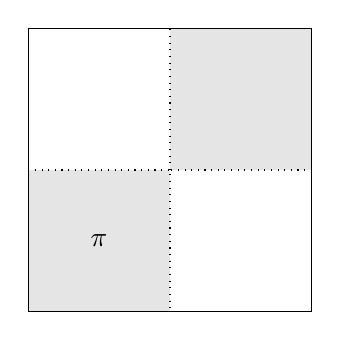
\begin{tikzpicture}[scale=.3]
        \draw[dotted, fill = black!10] 
              (0,6) -- (6,6) -- (6,0) -- (0,0) -- cycle;
        \draw[dotted, fill = black!10] 
              (6,6) -- (6,12) -- (12,12) -- (12,6) -- cycle;
        \draw (0,0) -- (12,0) -- (12,12) -- (0,12) -- cycle;
        \node at (3,3) {$\pi$};
        \node at (9,9) {$\sg$};
      \end{tikzpicture}
      \hspace{4pc}
      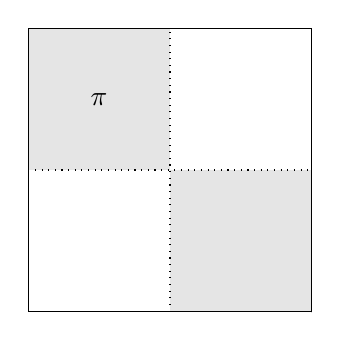
\begin{tikzpicture}[scale=.3]
        \draw[dotted, fill = black!10] 
              (0,6) -- (6,6) -- (6,12) -- (0,12) -- cycle;
        \draw[dotted, fill = black!10] 
              (6,0) -- (6,6) -- (12,6) -- (12,0) -- cycle;
        \draw (0,0) -- (12,0) -- (12,12) -- (0,12) -- cycle;
        \node at (3,9) {$\pi$};
        \node at (9,3) {$\sg$};
      \end{tikzpicture}

      \caption{The plots of $\pi \dsum \sg$ and $\pi \ssum \sg$, respectively.}
      \label{prelim:fig:sums}
    \end{figure}

    These definitions will prove essential when describing permutation
    classes. In his thesis~\cite{SteveWaton2007}, Waton describes and explores
    classes defined entirely by points plotted on specified geometric shapes.
    We focus here, however, on more general classes. 

    Direct sums and skew sums are simple examples of the so called
    \emph{inflation} operation. A non-geometric definition of inflation is
    technical and unillustrative, but is natural when viewed as an operation of
    permutation plots. Before defining inflations, we need another definition
    which will itself prove useful. 

    \begin{definition}\label{prelim:def:interval}
      Let $\pi = \pi_1 \pi_2 \dots \pi_n \in \S_n$. An \emph{interval} of
      $\pi$ is a contiguous sequence of entries $\pi_i \pi_{i+1} \dots
      \pi_{i+k}$ whose values form a contiguous sequence of integers. 
    \end{definition}

    For example, in the permutation $\pi = 2743516$, the third,
    fourth, and fifth entries ($435$) form an interval. 
    Every permutation has an interval of size $n$ (the entire permutation) and
    intervals of size one (each entry).  Permutations which have only these
    trivial intervals are especially significant. 
    

    \begin{definition} \label{prelim:def:simple}
      An permutation $\pi \in \S_n$ whose only intervals have size $1$ and $n$ is
      called \emph{simple}. 
    \end{definition}
    
    Simple intervals are useful for describing permutation classes,
    as we will see.  Monotone intervals will be investigated further in
    Chapters~\ref{chap:polyclass} and~\ref{chap:fixpat},
    and simplicity will be a major topic of Chapter~\ref{chap:involutions}. We
    can now define inflations, which will used throughout this dissertation. 

    \begin{definition}\label{prelim:def:inflation}
      Let $\pi \in S_n$, and let $\alp_1, \alp_2 \dots \alp_n$ be 
      permutations of any length. The \emph{inflation} of $\pi$ by the
      permutations $\alp_i$ is defined as the permutation obtained by replacing
      the $i$th entry of $\pi$ with an interval which is order isomorphic to
      the permutation $\alp_i$.  This inflation is denoted 
      $$ \pi[\alp_1, \alp_2, \dots \alp_n].$$
    \end{definition}

    \begin{figure}[t] \centering
      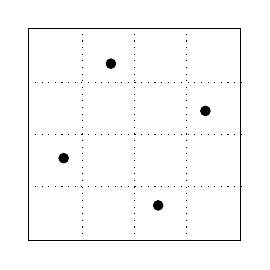
\begin{tikzpicture}[scale=.3]
        \draw (.5,.5) -- (9.5,.5) -- (9.5,9.5) -- (.5,9.5) -- cycle;
        \foreach \i in {2.8, 5, 7.2}{
          \draw[dotted] (.5,\i) -- (9.5, \i);
          \draw[dotted] (\i,.5) -- (\i, 9.5);
        }
        \draw[fill=black] (2, 4) circle (2mm);
        \draw[fill=black] (4, 8) circle (2mm);
        \draw[fill=black] (6, 2) circle (2mm);
        \draw[fill=black] (8,6) circle (2mm);
      \end{tikzpicture}
      \hspace{1pc}
      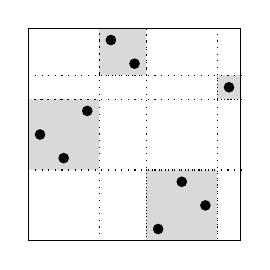
\begin{tikzpicture}[scale=.3]
        % \draw[fill=black!15] (.75,6.25)--(3.25,6.25)--(3.25,3.75)--(.75,3.75)--cycle;
        % \draw[fill=black!15] (3.75,9.25)--(5.25,9.25)--(5.25,7.75)--(3.75,7.75)--cycle;
        % \draw[fill=black!15] (5.75,3.25)--(8.25,3.25)--(8.25,.75)--(5.75,.75)--cycle;
        % \draw[fill=black!15] (8.75,7.25)--(9.25,7.25)--(9.25,6.75)--(8.75,6.75)--cycle;


        \draw[fill=black!15, dotted] 
            (.5,3.5)--(3.5,3.5)--(3.5,6.5)--(.5,6.5)--cycle;
        \draw[fill=black!15, dotted] 
            (3.5,7.5)--(5.5,7.5)--(5.5,9.5)--(3.5,9.5)--cycle;
        \draw[fill=black!15, dotted] 
            (5.5,.5)--(8.5,.5)--(8.5,3.5)--(5.5,3.5)--cycle;
        \draw[fill=black!15, dotted] 
            (8.5,6.5)--(9.5,6.5)--(9.5,7.5)--(8.5,7.5)--cycle;

        \draw (.5,.5) -- (9.5,.5) -- (9.5,9.5) -- (.5,9.5) -- cycle;
        \foreach \i in {3.5, 5.5, 8.5}{
          \draw[dotted] (\i,.5) -- (\i, 9.5);
        }
        \foreach \i in {3.5, 6.5, 7.5}{
          \draw[dotted] (.5,\i) -- (9.5, \i);
        }
        \foreach \y [count = \x] in {5,4,6,9,8,1,3,2,7}
          \draw[fill = black] (\x,\y) circle (2mm);
      \end{tikzpicture}
      \hspace{1pc}
      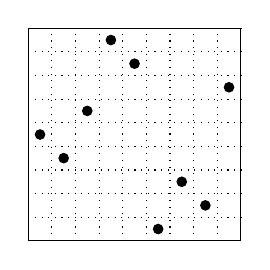
\begin{tikzpicture}[scale=.3]
      \draw (.5,.5) -- (9.5,.5) -- (9.5,9.5) -- (.5,9.5) -- cycle;

        \foreach \y [count = \x] in {5,4,6,9,8,1,3,2,7}{
          \draw[fill = black] (\x,\y) circle (2mm);
          \draw[dotted] (\x + 0.5, 0.5) -- (\x + 0.5, 9.5);
          \draw[dotted] (0.5, \x + 0.5) -- (9.5, \x + 0.5);
          }
    
      \end{tikzpicture}
      \caption[The simple permutation $2413$ and its inflation]{
                The simple permutation $2413$ and its inflation
                $2413[213, 21, 132, 1] = 546\ 98\ 132\ 7$.} 
      \label{prelim:fig:inflation}
    \end{figure}

    For example, for any two permutations $\pi$ and $\sg$, $\pi \dsum \sg =
    12[\pi, \sg]$ and $\pi \ssum \sg = 21[\pi, \sg]$. A more complicated
    example is shown in Figure~\ref{prelim:fig:inflation}. While simple
    permutations and inflations are useful for working with and describing
    permutations, their true utility is illustrated in the following theorem,
    which has generalizations to a wider range of combinatorial
    objects~\cite{SubsDecomp}. 


    % TODO: is this really necessary?
    % Note that in the literature, inflations by empty permutations are
    % generally not allowed. Throughout this document (and especially in
    % Chapter~\ref{chap:polyclass}), however, we go against tradition and allow
    % inflations by empty permutations, except where specified. This departure
    % is motivated partly by the fact that the set of all inflations of a
    % permutation (if we allow empty permutations) forms a permutation class.
    % We therefore define a \emph{proper} inflation of a permutation $\pi$
    % to be one in which each entry of $\pi$ is inflated by at least one
    % element. Allowing empty inflations will be useful in geometric class
    % descriptions. 

    \begin{theorem}[Substitution Decomposition~\cite{Brignall2008}]
      \label{thm:subsdecomp}
      Every permutation $\pi$ can be written as the inflation of a
      unique simple permutation. Further, if $\pi = \sg[\alp_1, \dots \alp_m]$,
      where each $\alp_i$ is a permutation of length $\geq 1$ and
      $m \geq 4$, then the permutations $\alp_i$ are uniquely determined as
      well. 
    \end{theorem}



\section{Dyck Paths and the Catalan Numbers}

    Before exploring two examples of permutation classes, we take a brief
    detour and investigate another set of combinatorial objects known as 
    \emph{Dyck paths}. These paths will be used throughout this dissertation,
    and provide a convenient and flexible means of encoding recursive and
    structural information. 
    
    These paths are enumerated by the so-called
    \emph{Catalan numbers}, a ubiquitous and useful sequence of integers.
    Stanley~\cite{Stanley2} has famously collected a series a sixty-six
    examples of combinatorial objects, each enumerated by these numbers. Their
    pervasiveness is due in part to their multiple recursive descriptions. 
    

  \subsection{Paths on the Integer Lattice}
    
    At its most formal, a \emph{Dyck path} of semilength $n$ is a sequence
    $\vec v_1, \vec v_2, \dots \vec v_{2n}$ of vectors $ \vec v_i \in
    \{\vect{1,1}, \vect{1,-1}\}$, satisfying $ \sum_{n=1}^{2n} \vec v_i =
    \vect{2n, 0}$ and, for all integers $k \in [2n]$ and $\vect{x,y} =
    \sum_{n=1}^k \vec v_i$, we have that $y \geq 0$. 

    As usual, a more intuitive definition will be useful. 
    Suppose that, starting from the point $(0,0) \in \mathbb{R}^2$, we want to
    travel to the point $(2n,0)$. Suppose further that are only allowed to walk
    diagonally northeast 
    (from a point $(x,y)$ to $(x+1, y+1)$) or southeast (from a point $(x,y)$
    to $(x+1, y-1)$). 
    Call a northeast step an \emph{upstep} and a southeast step a
    \emph{downstep}. The total number of walks from $(0,0)$ to $(2n,0)$ is then
    $\binom{2n}{n}$, since the number of up steps must equal the number of down
    steps, and so we need only specify which of the $2n$ steps are up. Dyck
    paths can now be defined as follows. 

    \begin{definition}\label{prelim:def:dyckpath}
      A \emph{Dyck path} of semilength $n$ (or of length $2n$) is path $p =
      s_1s_2 \dots s_{2n}$ from $(0,0)$ to $(2n,0)$ using the steps $u =
      \vect{1,1}$ and $d = \vect{1,-1}$ which \emph{never passes below the
      line $y=0$}. 
    \end{definition}

    These paths can be represented as a string of symbols from the alphabet
    $\{u,d\}$, representing upsteps and downsteps, respectively. The path $p =
    uuuddududduuddd$ is shown in Figure~\ref{prelim:fig:dyckpath}. 

    \begin{figure}[t]\centering
      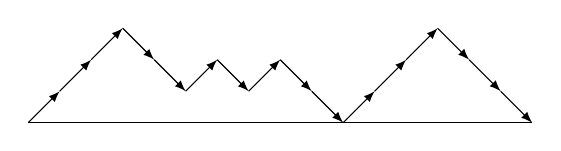
\begin{tikzpicture} [scale = .4]
        \draw (0,0) -- (16,0);
        \draw[->, >= latex] (0,0) -- (1,1);
        \draw[->, >= latex] (1,1) -- (2,2);
        \draw[->, >= latex] (2,2) -- (3,3);
        \draw[->, >= latex] (3,3) -- (4,2);
        \draw[->, >= latex] (4,2) -- (5,1);
        \draw[->, >= latex] (5,1) -- (6,2);
        \draw[->, >= latex] (6,2) -- (7,1);
        \draw[->, >= latex] (7,1) -- (8,2);
        \draw[->, >= latex] (8,2) -- (9,1);
        \draw[->, >= latex] (9,1) -- (10,0);
        \draw[->, >= latex] (10,0) -- (11,1);
        \draw[->, >= latex] (11,1) -- (12,2);
        \draw[->, >= latex] (12,2) -- (13,3);
        \draw[->, >= latex] (13,3) -- (14,2);
        \draw[->, >= latex] (14,2) -- (15,1);
        \draw[->, >= latex] (15,1) -- (16,0);
      \end{tikzpicture}
      \caption{A Dyck path of semilength $8$.}
      \label{prelim:fig:dyckpath}
    \end{figure}

  \subsection{Enumerating Dyck Paths}
    
    
    Dyck paths are a fundamental combinatorial object, and their properties
    have been studied extensively~\cite{Chapman1999, Deutsch1999, Denise1995}. 
    Their well understood structure makes them (and their generalizations) a
    useful intermediate object for building bijections between other
    objects~\cite{Claesson2008, bloomvince}. To illustrate their recursive
    structure, we derive their enumeration here. 

    In order to count Dyck paths, we first need to consider their structure,
    and how they can be broken down into smaller pieces. We focus on two
    separate decompositions, which lead to two different recursive
    descriptions, each of which leads to the Catalan numbers. 

    First, let $p = s_1 s_2 \dots s_{2n}$ be a Dyck path, and let $s_i$ be the
    first step which brings it back to the line $y = 0$. Such a step must
    exist, since $s_{2n}$ always ends at this line. It follows
    then that $i$ is even, $s_1 = u$, $s_i = d$, and $s_{i+1} s_{i+2} \dots
    s_{2n}$ is a Dyck path of length $2n-i$. 
    Further, since $s_i$ is the \emph{first} time
    the path touches the line $y=0$, each of the steps $s_2, s_3, \dots
    s_{i-1}$ have a height greater than or equal to $1$, which implies that
    $s_2 s_3 \dots s_{i-1}$ is a Dyck path. This implies that for every Dyck
    path $p$, there exist two smaller Dyck paths $p_1, p_2$ such that $$ p = u
    p_1 d\ p_2 .$$

    It follows that if $\cP$ is the \emph{language} of Dyck paths (i.e., the
    set of all strings of the letters $u,d$ which represent valid Dyck paths),
    then $\cP = u \cP d \cP + \eps$, where the $\eps$ represents the empty
    path. This leads immediately to a generating function relation: if we let
    $c_n$ be the number of Dyck paths of semilength $n$ and $C(z) = \sum_{n\geq
    0} c_n z^n$, then this relation leads to the equation 

    \begin{equation}  \label{prelim:eqn:firstpass}   
      C(z) = z C(z)^2 + 1. 
    \end{equation}

    Before investigating further, we present an alternate decomposition. Let $p
    = s_1 s_2 \dots s_{2n}$ be a Dyck path, and let $i_1, i_2, \dots i_k$ be
    all of the indices with the property that the step $s_i$ ends on the line
    $y=0$. It follows then that each subword $s_{i_j + 1} s_{i_j + 2} \dots
    s_{i_{j+1} -1}$ stays above the line $y=1$, and is therefore itself a Dyck
    path. Therefore, for all Dyck paths $p$, there exist some integer $k$ and
    Dyck paths $p_1, p_2, \dots p_k$ such that 
    $$ p = u p_1 d\  u p_2 d\  \dots u p_k d.$$
    This gives an alternate relation for the generating function $C(z)$
    enumerating Dyck paths:
    
    \begin{equation} \label{prelim:eqn:allpass}
      C(z) = 1 + zC(z) + z^2 C(z)^2 + z^3 C(z)^3 + \dots = \frac{1}{1 - zC(z)}.
    \end{equation}

    The equivalence of equations~\ref{prelim:eqn:allpass}
    and~\ref{prelim:eqn:firstpass} is immediately obvious --- one can be
    rearranged into the other.
    It follows then that these two seemingly different recursions are in fact
    equivalent, and so any object exhibiting either of these recursive
    descriptions are counted by the same numbers. 
    With Dyck paths, both recurrences are clear;
    with other objects, however, they are less transparent. Dyck paths are
    useful in part because of the simplicity of their decompositions, and
    Catalan numbers are ubiquitous because they capture so many of these
    recursions. 

  \subsection{The Catalan Numbers}
  \label{prelim:sub:catalan}
    
    The generating function presented above
    (equation~\ref{prelim:eqn:firstpass}) can be solved using the quadratic
    formula, yielding the following (note that the quadratic formula actually
    yields two solutions, but we discard the one which does not have a series
    expansion with positive integer coefficients) 

    \begin{equation} \label{eqn:catalan-gfn}
      C(z) = \sum_{n \geq 0} c_n z^n = \frac{1 - \sqrt{1 - 4z}}{2z}.
    \end{equation}

    The first few coefficients in the expansion of $C(z)$ are
    $1,1,2, 5, 14, 42, 132, \dots$, and are \OEIS{A000108}.  The generating
    function recurrence $C(z) = zC(z)^2 + 1$ translates to $c_0 =1$ and
    $c_{n+1} = \sum_{k=0}^n c_{k} c_{n-k}$, and this uniquely defines this
    sequence.  The binomial theorem can be used to obtain an exact formula for
    $c_n$ from equation~\ref{eqn:catalan-gfn} above:

    \begin{equation} \label{eqn:catalan-exact}
      c_n = \frac{1}{n+1} \binom{2n}{n} = \binom{2n}{n} - \binom{2n}{n-1}.
    \end{equation}

    We note that the generating function presented above
    (equation~\ref{eqn:catalan-gfn}) has a singularity at $z=1/4$. It follows
    that, when expanded as a power series about $z=0$, $C(z)$ has a radius of
    convergence of $1/4$. The exponential growth rate of a sequence is equal to
    the reciprocal of the radius of convergence, which implies that $\limn
    \sqrt[n]{c_n} = 4$. 
    While Stirling's approximation for the factorials gives a simpler means of
    calculating this growth rate (and allow for the derivation of the
    subexponential growth rate), analytic techniques, summarized in the
    textbook of Flajolet and Sedgewick~\cite{flajolet}, provide a wide
    framework for deriving these exponential growth rates.




\section{Four Case Studies}


  The advantage to this geometric focus is best illustrated through 
  examples. In this section we present four case studies, each of which
  corresponds roughly to the subject of a later chapter. Together these provide
  motivation and a gentle introduction to the methods used throughout this
  dissertation.
  
  We begin by deriving the 
  enumeration of the classes of $132$- and $123$-avoiding permutations. Though
  they share the same enumeration, these two classes present starkly different
  decompositions. We then combine these ideas and explore the class of
  \emph{$123$- and $231$}-avoiding permutations, motivating the investigation
  of polynomial permutation classes. Finally, we examine an example of the use of
  probabilistic techniques and structural decomposition in finding
  statistical information about classes. 



  \subsection{Permutations Avoiding 132}
  \label{prelim:sec:av132}

    
    We start with the enumeration of the class $\Av (132)$.  The study of
    simples within a permutation class has been a deep and productive line of
    research in recent years~\cite{Brignall2008, Atkinson2005, Brignall2007}.  
    Further, this investigation has seen numerous applications in the
    enumeration of classes~\cite{pantone2013,pantone2014, Albert2012}.
    %
    % TODO add line about 'numerous applications' and cite more people
    %
    While the vast majority of this machinery is not needed for the class $\Av
    (132)$, but in the interest of exposition we hit a small nail with a large
    hammer.  The enumeration of a class using its simples is the core idea of
    Chapter~\ref{chap:involutions}, where we apply it to sets of
    pattern-avoiding involutions. 
    
    A plot of a permutation within $\Av (132)$ has strict restrictions: every
    element to the left of the highest point must be higher than every element
    to the right, since otherwise we would have a $132$ pattern with the
    highest element playing the role of the 3. This highest element then
    divides the plot into two sides. It follows that every entry after the
    peak forms an interval, which implies that the only simples in $\Av (132)$
    are $\{1, 12, 21\}$. 


    By describing the simple permutations in the class, we can often obtain a
    full enumeration. The class $\Av (132)$ is uncomplicated enough to be
    described entirely using direct and skew sums, but it falls into a larger
    set of classes, those which have only finitely many simple permutations.
    Such permutation classes posess a number of useful properties, including
    the following theorem, due to Albert and Atkinson. 

    \begin{theorem}[Albert, Atkinson~\cite{Atkinson2005}]
      If a class contains only finitely many simple permutations, then its
      enumeration is given by an algebraic generating function. 
    \end{theorem}

    In addition to theoretical results, the investigation of simple
    permutations and decomposition has led to practical enumeration techniques.
    Once the simples of a class have been obtained, one needs only determine
    the manner in which each simple can be inflated in order to fully describe
    the class. While much of this work has focused on enumerating classes, it
    can also be used to obtain statistical information about the class.
    Section~\ref{prelim:sec:ascents-example} gives an introductory example to
    this technique, while Chapter~\ref{chap:expat} explores the concept
    further. 

    Returning now to the class $\Av(132)$, note that arbitrary inflations of
    the simple permutations $\{1, 12, 21\}$ do not lead to $132$-avoiding
    permutations. Letting $\pi \in \Av(132)$, recall that every entry after the
    maximal entry must have a smaller value than every entry before. The
    substitution decomposition (Theorem~\ref{thm:subsdecomp}) implies that 
    each permutation can be defined as an inflation of precisely one of these:
    the simple permutation $1$ can only be inflated to the length $1$
    permutation, inflations of
    $12$ are the sum-decomposable elements, and the skew-decomposable elements
    are the inflations of $21$. 
    
    For an inflation of $12$, the $2$ can only be inflated by an
    increasing run of entries, or else would contain a $21$ pattern, creating a
    $132$ occurrence with any entry of the inflation of the $1$, which can be
    inflated by any $132$-permutation.  Recall that the substitution
    decomposition does not guarantee uniqueness when inflating the simple
    permutations $12$ and $21$, so we have to be careful. To ensure uniqueness,
    only allow the $2$ of $12$ to be inflated by a single element (if there is
    an increasing run, take it to be part of the $1$). 


    Finally, when inflating $21$, the $1$ can be inflated by any
    $132$-permutation, while the $2$ can be inflated by any $132$-avoiding
    permutation which ends in its last element, which can be represented as the
    direct sum of a $132$-avoiding permutation (or the empty permutation) with
    the permutation $1$. We express this as follows, letting $\C$ denote $\Av
    (132)$ and $\eps$ denote the empty permutation:

    $$ \C =  1\big[1\big] \ \bigcup \ 12\big[\C, 1\big] \ \bigcup \
        21\big[(\C \cup \eps) \dsum 1, \C\big]. $$

    Letting $f$ denote the generating function $\sum_{n \geq 0} |\Av_n (132)|
    z^n$, this leads to the following expression

    $$ f =  z + fz  + z(f+1)f .$$

    Solving for $f$ using the quadratic formula gives that $f$ is the generating
    function for the Catalan numbers with the constant term subtracted off.
    This gives an exact formula for the enumeration of $\Av (132)$, 
    as originally derived by Knuth~\cite{Knuth}. 
    
    \begin{theorem} \label{prelim:thm:av132}
      The number of permutations of length $n$ avoiding $132$ is the $n$th Catalan
      number $c_n = \frac{1}{n+1}\binom{2n}{n}$. 
    \end{theorem}


    Note that this result can be obtained using more elementary methods. 
    It follows that a permutation is $132$-avoiding if and only if it can be
    written as $(\pi \dsum 1) \ssum \sg$, where $\pi$ and $\sg$ are
    $132$-avoiding permutations (or empty). Applying this characterization
    iteratively provides a recursive description of the $132$-avoiding
    permutations, shown in Figure~\ref{prelim:fig:av132-first}, and in fact
    characterizes this class.


    \begin{figure}[t] \centering
      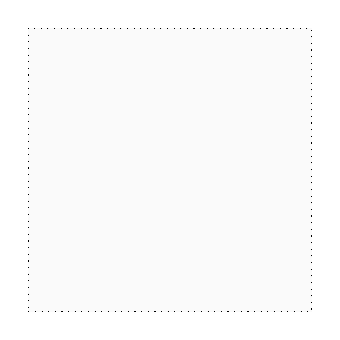
\begin{tikzpicture}[scale = .3]
        \draw[dotted, fill=black!2] (0,0) -- (12,0) -- (12,12) -- (0, 12) -- cycle;
        \node at (6,6) {$\C$};

      \end{tikzpicture}
      \hspace{1pc}
      \raisebox{4pc}{$= $}
      \hspace{1pc}
      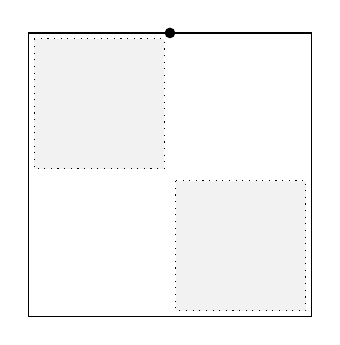
\begin{tikzpicture}[scale = .3]
        \draw (0,0) -- (12,0) -- (12,12) -- (0, 12) -- cycle;

        \draw[fill = black] (6,12) circle (2mm);
        \draw[dotted, fill=black!5] (.25,11.75) -- (5.75,11.75) 
                              -- (5.75,6.25) -- (.25,6.25) -- cycle;
        \draw[dotted, fill=black!5] (6.25,5.75) -- (11.75,5.75) 
                              -- (11.75,.25) -- (6.25,.25) -- cycle;
        \node at (3,9) {$\C$};
        \node at (9,3) {$\C$};
      \end{tikzpicture}
      \hspace{1pc}
      \raisebox{4pc}{$= $}
      \hspace{1pc}
      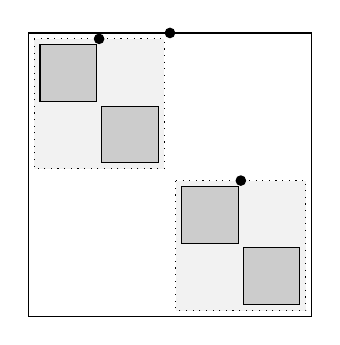
\begin{tikzpicture}[scale = .3]
        \draw (0,0) -- (12,0) -- (12,12) -- (0, 12) -- cycle;

        \draw[fill = black] (6,12) circle (2mm);
        \draw[dotted, fill=black!5] (.25,11.75) -- (5.75,11.75) 
                              -- (5.75,6.25) -- (.25,6.25) -- cycle;
        \draw[dotted, fill=black!5] (6.25,5.75) -- (11.75,5.75) 
                              -- (11.75,.25) -- (6.25,.25) -- cycle;
        
        \draw[fill=black] (3, 11.75) circle (2mm);
        \draw[fill=black] (9, 5.75) circle (2mm);

        \draw[fill=black!20] (.5, 11.5) -- (2.9,11.5)
                              -- (2.9, 9.1) -- (.5,9.1) -- cycle;
        \draw[fill=black!20] (3.1, 8.9) -- (5.5,8.9)
                              -- (5.5, 6.5) -- (3.1,6.5) -- cycle;

        \draw[fill=black!20] (6.5, 5.5) -- (8.9, 5.5) 
                              -- (8.9, 3.1) -- (6.5, 3.1) -- cycle;
        \draw[fill=black!20] (9.1, 2.9) -- (11.5, 2.9) 
                              -- (11.5, .5) -- (9.1, .5) -- cycle;

        \node at (1.7, 10.3) {$\C$};
        \node at (4.3, 7.7) {$\C$};
        \node at (7.7, 4.3) {$\C$};
        \node at (10.3, 1.7) {$\C$};


      \end{tikzpicture}
    \caption{A geometric description of the class $\C = \Av 132$.}
    \label{prelim:fig:av132-first}
    \end{figure}
     

    This recursive decomposition can be used to generate a recursively defined
    bijection $\phi: \Av_n(132) \ra \cD_n$ from permutations in $\Av_n (132)$
    to Dyck paths of semilength $n$, thus reproving 
    Theorem~\ref{prelim:thm:av132} once again. Let $\pi \in \Av_n(132)$, and $\pi = (\pi_1
    \dsum 1) \ssum \pi_2$ be the decomposition defined above. Then define 
    $$\phi(\pi) = u \ \phi(\pi_1) \ d \ \phi(\pi_2).$$
    This recursive definition was originally presented by Knuth~\cite{Knuth}.
    For example, 
    $$ \begin{aligned}
      \phi(74352681) 
        &= u\phi(743526)d\phi(1) \\
        &= u (ud \phi(43526)) d ud \\
        &= uud (u\phi(4352)d) dud \\
        &= uudu (u\phi(43)d)\phi(2) dud\\
        &= uuduu (ud\phi(3))d (ud) dud \\
        &= uuduuud (ud) duddud \\
        &= uuduuududduddud \in \cD_n.
    \end{aligned} $$
    
    There is an alternate, non-recursive bijection $\varphi$, first presented
    in an alternate, non-geometric form by
    Krattenthaler~\cite{Krattenthaler2001},
    whose equivalence to the above definition follows from the work of Claesson
    and Kitaev~\cite{Claesson2008}. Let $\pi \in \Av_n(132)$, and define
    $\varphi(\pi)$ as follows. First, plot $\pi$ and define a lattice path from
    $(1,n)$ to $(n,1)$ using the steps $\{\vect{0,-1}, \vect{1,0}\}$. Take this
    to be the unique path using these steps which maximizes the area underneath
    the path, while remaining below and to the left of each entry of the
    plotted permutation. Finally, translate this to a Dyck path by mapping each
    $\vect{0,-1}$ to be an up step, and each $\vect{1,0}$ to be a down step.
    See Figure~\ref{prelim:fig:dyckbiject-geom} for an example. 

    \begin{figure}[t] \centering
      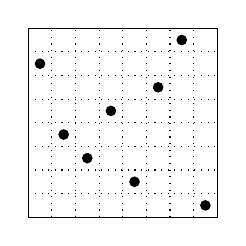
\begin{tikzpicture}[scale=.3]
        \draw (1,1) -- (1,9) -- (9,9) -- (9,1) -- cycle;
        \foreach \y [count = \x] in {7,4,3,5,2,6,8,1}{
          \draw[fill = black] (\x+.5,\y+.5) circle (2mm);
        }
        \foreach \i in {1, ...,9}{
          \draw[dotted] (\i,1) -- (\i,9);
          \draw[dotted] (1,\i) -- (9,\i);
        }
      \end{tikzpicture}
      \hspace{2pc}
      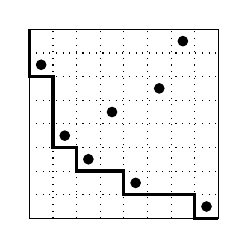
\begin{tikzpicture}[scale=.3]
        \draw (1,1) -- (1,9) -- (9,9) -- (9,1) -- cycle;
        \foreach \y [count = \x] in {7,4,3,5,2,6,8,1}{
          \draw[fill = black] (\x+.5,\y+.5) circle (2mm);
        }
        \foreach \i in {1, ...,9}{
          \draw[dotted] (\i,1) -- (\i,9);
          \draw[dotted] (1,\i) -- (9,\i);
        }
        \draw[very thick] (1,9) --++ (0,-2) --++ (1,0) --++ (0,-3)
                          --++ (1,0) --++(0,-1) --++(2,0) 
                          --++ (0,-1) --++ (3,0) --++(0,-1) 
                          --++ (1,0);
      \end{tikzpicture}
      \hspace{2pc}
      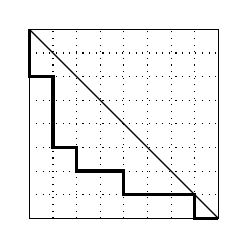
\begin{tikzpicture}[scale=.3]
        \draw (1,1) -- (1,9) -- (9,9) -- (9,1) -- cycle;
        \foreach \i in {1, ...,9}{
          \draw[dotted] (\i,1) -- (\i,9);
          \draw[dotted] (1,\i) -- (9,\i);
        }
        \draw (1,9) -- (9,1);
        \draw[very thick] (1,9) --++ (0,-2) --++ (1,0) --++ (0,-3)
                          --++ (1,0) --++(0,-1) --++(2,0) 
                          --++ (0,-1) --++ (3,0) --++(0,-1) 
                          --++ (1,0);
      \end{tikzpicture}
      \hspace{2pc}
      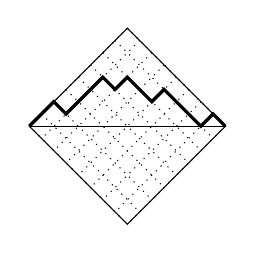
\begin{tikzpicture}[scale=.22]
      \begin{scope}[shift={(3,5)},rotate=-45, yscale=-1]
        \draw (1,1) -- (1,9) -- (9,9) -- (9,1) -- cycle;
        \foreach \i in {1, ...,9}{
          \draw[dotted] (\i,1) -- (\i,9);
          \draw[dotted] (1,\i) -- (9,\i);
        }
        \draw (1,9) -- (9,1);
        \draw[very thick] (1,9) --++ (0,-2) --++ (1,0) --++ (0,-3)
                          --++ (1,0) --++(0,-1) --++(2,0) 
                          --++ (0,-1) --++ (3,0) --++(0,-1) 
                          --++ (1,0);
        \end{scope}
        \end{tikzpicture}
    \caption{The construction of the Dyck path $\varphi(74352681)$.  }
                % The final step reflects the path across the
                % diagonal, and then rotates through an angle of $\pi/4$.} 
    \label{prelim:fig:dyckbiject-geom}
    \end{figure}



  \subsection{Permutations Avoiding 123}
  \label{prelim:sec:av123}

    Despite having the same enumeration, the class $\Av(123)$ presents a stark
    contrast to the class $\Av (132)$. First, there are infinitely many
    simple permutations in the class, which prevents us from using many of the
    tools from the previous example. Enumerating and describing these simples
    is the central idea of Chapter~\ref{chap:involutions}. We first present a
    bijective enumeration of the class, before analyzing the structure. 
    
    As a further example highlighting the benefit of the geometric viewpoint
    note that, remarkably, the bijection $\varphi$ described in
    Figure~\ref{prelim:fig:dyckbiject-geom} leads to a bijection
    $\varphi':\Av_n(123) \ra \cD_n$, using \emph{exactly the same description}.
    See Figure~\ref{prelim:fig:123biject} for an example. Note that
    $\varphi^{-1}
    \circ \varphi'$ is a bijection from $\Av_n (123)$ to $\Av_n (132)$, which is
    equivalent to the one presented by Simion and Schmidt~\cite{Simion1985},
    and shows that the locations of left-to-right minima has the same
    distribution in both classes. 

    \begin{figure}[t] \centering
      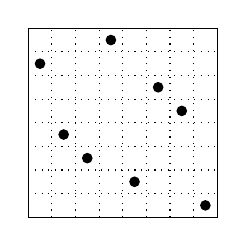
\begin{tikzpicture}[scale=.3]
        \draw (1,1) -- (1,9) -- (9,9) -- (9,1) -- cycle;
        \foreach \y [count = \x] in {7,4,3,8,2,6,5,1}{
          \draw[fill = black] (\x+.5,\y+.5) circle (2mm);
        }
        \foreach \i in {1, ...,9}{
          \draw[dotted] (\i,1) -- (\i,9);
          \draw[dotted] (1,\i) -- (9,\i);
        }
      \end{tikzpicture}
      \hspace{2pc}
      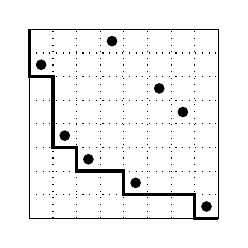
\begin{tikzpicture}[scale=.3]
        \draw (1,1) -- (1,9) -- (9,9) -- (9,1) -- cycle;
        \foreach \y [count = \x] in {7,4,3,8,2,6,5,1}{
          \draw[fill = black] (\x+.5,\y+.5) circle (2mm);
        }
        \foreach \i in {1, ...,9}{
          \draw[dotted] (\i,1) -- (\i,9);
          \draw[dotted] (1,\i) -- (9,\i);
        }
        \draw[very thick] (1,9) --++ (0,-2) --++ (1,0) --++ (0,-3)
                          --++ (1,0) --++(0,-1) --++(2,0) 
                          --++ (0,-1) --++ (3,0) --++(0,-1) 
                          --++ (1,0);
      \end{tikzpicture}
      \hspace{2pc}
      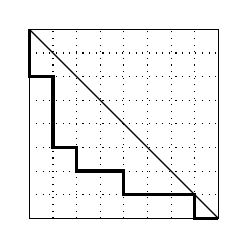
\begin{tikzpicture}[scale=.3]
        \draw (1,1) -- (1,9) -- (9,9) -- (9,1) -- cycle;
        \foreach \i in {1, ...,9}{
          \draw[dotted] (\i,1) -- (\i,9);
          \draw[dotted] (1,\i) -- (9,\i);
        }
        \draw (1,9) -- (9,1);
        \draw[very thick] (1,9) --++ (0,-2) --++ (1,0) --++ (0,-3)
                          --++ (1,0) --++(0,-1) --++(2,0) 
                          --++ (0,-1) --++ (3,0) --++(0,-1) 
                          --++ (1,0);
      \end{tikzpicture}
      \hspace{2pc}
      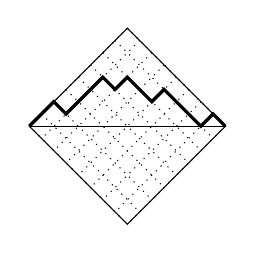
\begin{tikzpicture}[scale=.22]
      \begin{scope}[shift={(3,5)},rotate=-45, yscale=-1]
        \draw (1,1) -- (1,9) -- (9,9) -- (9,1) -- cycle;
        \foreach \i in {1, ...,9}{
          \draw[dotted] (\i,1) -- (\i,9);
          \draw[dotted] (1,\i) -- (9,\i);
        }
        \draw (1,9) -- (9,1);
        \draw[very thick] (1,9) --++ (0,-2) --++ (1,0) --++ (0,-3)
                          --++ (1,0) --++(0,-1) --++(2,0) 
                          --++ (0,-1) --++ (3,0) --++(0,-1) 
                          --++ (1,0);
        \end{scope}
        \end{tikzpicture}
    \caption{The construction of the Dyck path $\varphi'(74382651)$.
                }
    \label{prelim:fig:123biject}
    \end{figure}

    A modification of this bijection is central to Chapter~\ref{chap:expat},
    and will be used to count pattern \emph{occurrences} within the class.
    Dyck paths can be used to encode structural information about the
    permutations they represent, and can be easily enumerated. 


    \begin{figure}[t] \centering
      \begin{tikzpicture}[scale=.3]
        \foreach \y [count = \x] in {9,7,10,5,8,3,6,1,4}{
          \draw[fill = black] (\x+.5,\y+.5) circle (2mm);
        }

        \foreach \i in {1,2,3}
          \draw[fill = black] (10 + 0.4*\i, 2.2 - 0.4*\i) circle (.5mm);

      \end{tikzpicture}
    \caption{The decreasing oscillations.}
    \label{prelim:fig:oscillation}
    \end{figure}

    To see that $\Av (123)$ contains infinitely many simple permutations, we
    define the \emph{decreasing oscillations}, a family of simples which are
    contained within the class. Figure~\ref{prelim:fig:oscillation} gives a
    graphical description of these permutations. 
    Though the simples are not as easily described as in our previous example,
    $\Av(123)$ exhibits a different kind of geometric structure which will be
    equally useful. Since a $123$-avoiding permutation does not contain any
    three increasing entries, it follows that it can be written as the union of
    two decreasing sequences of entries. It follows further that we can
    partition the plot of such a permutation into an alternating sequence of
    monotone decreasing runs. We formalize this in
    Chapter~\ref{chap:involutions}, but for now present an diagram of the
    so-called \emph{staircase decomposition}~\cite{Albert2010, me-involutions}
    in Figure~\ref{prelim:fig:staircase}.


    \begin{figure}[t] \centering
      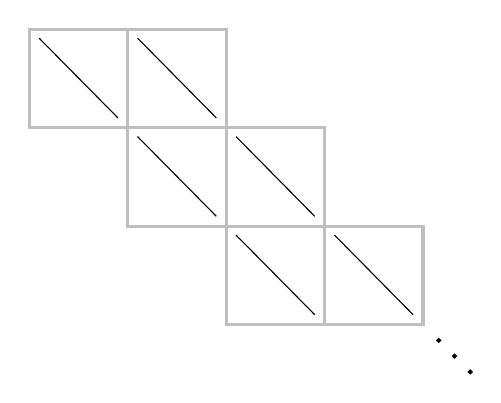
\begin{tikzpicture}[scale=.25]
        % draw the outer boxes, using a loop
        \foreach \x/\y in {0/0, 5/0, 5/-5, 10/-5, 10/-10, 15/-10}{
          \draw[very thick, color=lightgray] (\x, \y) rectangle (\x + 5, \y + 5);
          \draw (\x+.5, \y+4.55) -- (\x + 4.5, \y + .5 );
        }
        \foreach \i in {1,2,3}
          \draw[fill = black] (20 + 0.8*\i, -10 - 0.8*\i) circle (1mm);

      \end{tikzpicture}
    \caption{The class $\Av(123)$ is precisely those permutations which can be
             plotted on descending lines of the diagram.}
    \label{prelim:fig:staircase}
    \end{figure}

    This decomposition will be used to enumerate and describe the simple
    permutations within the class, which will then be used to enumerate pattern
    avoiding involutions in Chapter~\ref{chap:involutions}. 
    We present one final method of enumerating the class $\Av(123)$, by
    inflating the (infinitely many) simples. In Chapter~\ref{chap:involutions}
    we use the staircase decomposition to enumerate the simples of the class,
    and find that their generating function
    (equation~\ref{eqn:genfcn-simple123perms}) is given by 
    $$ f = \sum_{\substack{ \sg \in \Av(123) \\ \sg \text{ simple}}}
        z^{|\sg|} = \frac{1 - z - \sqrt{1 - 2z - 3z^2}}{2z} .$$

    Each entry of a simple permutation in the class can be inflated only by
    decreasing runs, whose generating functions are given by $\frac{z}{1-z}$.
    It follows then that, since each $z$ in the above generating function
    represents an entry of a simple permutation, replacing $z$ by
    $\frac{z}{1-z}$, we obtain the generating function for all permutations of
    the class. Indeed, after simplifying, we find that this composition gives
    the generating function for the Catalan numbers, with the constant term
    (representing the empty permutation) removed: 
    $$ f\left(\frac{z}{1-z}\right) = \frac{1 - 2z - \sqrt{1-4z}}{2z}.$$



  \subsection{Permutations Avoiding 123 and 231}
  \label{prelim:sec:av123+231}

    Our next example enumerates the class $\Av(123, 231)$ of
    permutations which avoid both $123$ and $231$, using a structural
    description of the class. This example motivates the exploration of the
    \emph{polynomial classes} (the classes whose enumeration is given by a
    polynomial). This will be investigated more fully in
    Chapter~\ref{chap:polyclass}, where an algorithm will be presented which,
    given a structural description, enumerates the class. 

    Since we have already shown that the only simples in the class $\Av (231)$
    are $\{1, 12, 21\}$ (because it is a symmetry of $\Av(132)$), the fact that
    $\Av(123, 231) \subset \Av(231)$ implies that these are the same simples in
    $\Av(123, 231)$. The added restriction of avoiding $123$ changes the way
    these simples can be inflated. Both entries of $12$ can only be inflated by
    decreasing runs, to avoid constructing an occurrence of $123$. Finally, the
    first entry of a $21$ can be inflated only by a decreasing run (to avoid
    $231$), while the second can be inflated by any element from the class. 
    
    After accounting for uniqueness, it follows that every permutation in the
    class can be obtained by inflating the permutation $312$ with (possibly
    empty) descending permutations. Therefore, this class is precisely those
    permutations which can be drawn on the diagram shown in
    Figure~\ref{prelim:fig:polygrid}


    \begin{figure}[t] \centering
      \begin{tikzpicture}[scale=.35]
        \draw (0,0) -- (12,0) -- (12,12) -- (0,12) -- cycle;
        \draw[dotted] (4,0) -- (4,12);
        \draw[dotted] (8,0) -- (8,12);
        \draw[dotted] (0,4) -- (12,4);
        \draw[dotted] (0,8) -- (12,8);
        \draw (0,12) -- (4,8);
        \draw (4,4) -- (8,0);
        \draw (8,8) -- (12,4);
      \end{tikzpicture}
    \caption{The class $\Av(123, 231)$ is precisely those permutations which can be
             plotted on descending lines of the diagram.}
    \label{prelim:fig:polygrid}
    \end{figure}

    This is a simple example of a \emph{grid class}
    %TODO cite murphyvatter
    ~\cite{MurphyVatter}, a useful concept which has produced many new
    enumerations in recent years. It is known~\cite{SophieVince,GridClasses},
    and is presented formally in Theorem~\ref{polyclass:thm:tfae}, that a
    permutation class is enumerated by a polynomial if and only if it is a
    union or intersection of classes which can be represented with such a
    diagram, with only one nonempty cell per row and column. 

    Returning to Figure~\ref{prelim:fig:polygrid}, it is trivial to enumerate
    those permutations which have at least one element in each block: the
    generating function for a single block is $z/(1-z)$, and so the
    generating function for those with no empty blocks are
    $z^3/(1-z)^3$. If the first block is empty, then we have the
    generating function $z^2/(1-z)^2$. If either the second or third
    block is empty, the entire permutation is a single decreasing run, with
    generating function $z/(1-z)$. Therefore, the generating function for
    the entire class is simply the sum of these three:

    \begin{equation} \label{prelim:eqn:polyclass}
      \sum_{n \geq 1} |\Av_n (123,231)| z^n = 
        \frac{z^3}{(1-z)^3} + \frac{z^2}{(1-z)^2} + \frac{z}{1-z} =
        \frac{z^3- z^2 + z}{(1-z)^3}.
    \end{equation}

    Equation~\ref{prelim:eqn:polyclass} expanded using the binomial theorem to
    produce an exact equation for the number of permutations of each length in
    the class. 

    $$ | \Av_n (123, 231) | = \frac{n^2 - n + 2}{2} = \binom{n}{2} + 1.$$

    More complicated decompositions lead to a number of technical obstacles, but
    this same general idea can be used to calculate the polynomials enumerating all
    such classes. This will be presented in Chapter~\ref{chap:polyclass}, and
    an implementation of the algorithm is available
    online~\cite{polyclass-algo}. 

  \subsection{Ascents in 132-Avoiding Permutations}
  \label{prelim:sec:ascents-example}
  
    We end this chapter with an illustrative example which utilizes a class's
    structural decomposition to investigate the distribution of a permutation
    statistic. This example, while relatively simple, serves to showcase the
    techniques which will be used throughout the following chapters, and
    is particularly pertinent to Chapter~\ref{chap:expat}.
    
 
    A \emph{permutation statistic} is any function $\chi: \S_n \ra \bR$. In
    practice, we often consider statistics that map from permutations to
    non-negative integers which capture some structural trait of the
    permutation. Examples include the location of the largest element, number
    of cycles, value of the first entry, and number of inversions. In this
    section we consider the number of ascents of a permutation. An
    \emph{ascent} of a permutation $\pi = \pi_1 \pi_2 \dots \pi_n$ is an index
    $i$ such that $\pi_i < \pi_{i+1}$, and the number of ascents in a
    permutation $\pi$ is denoted $\asc(\pi)$. 


    For a given permutation $\pi$ of length $n$, it follows that $\asc(\pi) \in \{0, 1,
    \dots n-1\}$. If $i$ is an ascent of $\pi$ then $i$ is a descent of
    $\pi^c$, and so the number of permutations of lengh $n$ with $k$ ascents is equal to
    the number of such permutations with $k$ descents (or $n - k - 1$ ascents).
    This implies in particular that the \emph{average} number of ascents in a
    randomly selected permutation from $\S_n$ is $(n-1)/2$. When we restrict to a
    proper permutation class, however, the distribution can be more difficult
    to compute. 

    For a finite set $S$ of permutations and a statistic $f$, the
    \emph{generating polynomial} for $f$ on $S$ in indeterminate $u$ is 
    $$ \sum_{\pi \in S} u^{f(\pi)}.$$
    For example, if $\S_3 = \{123, 132, 213, 231, 312, 321\}$ then the generating
    polynomial for the number of ascents is $u^2 + 4u + 1$, since there is one
    permutation with two ascents, four with one ascent, and one permutation
    with no ascents. There is one crucial observation: if we take the
    derivative (with respect to $u$) of the generating polynomial and set $u=1$
    we obtain a weighted sum which evaluates to the expected value, or average,
    of the statistic on $S$. Further, by differentiating twice before setting
    $u=1$, and then dividing by two, we obtain the first factorial moment of
    the statistic, which can be used to compute the variance. This process can
    be iterated to calculate higher moments of the distribution. 

    Extending to permutation classes, let $|\pi|$ denote the length of a
    permutation $\pi$ and define the generating function for a statistic $f$
    across a class $\C$ as
    $$ \sum_{\pi \in \C} z^{|\pi|} u^{f(\pi)}.$$
    The coefficient of $z^n$ in this bivariate generating function is precisely
    the generating polynomial for the statistic $f$ on the set $\C_n$, and so
    it follows that by differentiating with respect to $u$ and plugging in
    $u=1$, we can obtain generating functions whose coefficients represent the
    moments of the distribution on $\C_n$. Asymptotic analysis can then be used
    to compute the limiting distribution as $n$ approaches infinity. 



    Throughout this section, let $a_{n,k}$ be the number of $132$-avoiding
    permutations of length $n$ which contain exactly $k$ ascents, and let
    $$f(z,u) = \sum_{\pi \in \Av(132)} z^{|\pi|} u^{\asc(\pi)} = 
              \sum_{n \geq 0} \sum_{k \geq 0} a_{n,k} u^k z^n.$$

    Our goal is to derive a closed expression for $f$, and use this to analyze
    the distribution of descents across $\Av(132)$. Consider the recursive
    description of the class, shown in Figure~\ref{prelim:fig:av132-first}, and
    let $\pi = (\ro \dsum 1) \ssum \sg$ be a $132$-avoiding permutation. It
    follows that the number of ascents of $\pi$ is equal to the sum of ascents
    in $\ro$ and $\sg$, plus one \emph{if} $\ro$ is nonempty (otherwise the
    permutation starts with its biggest entry).
    This relationship leads to the following functional equation. 

    $$ f = zf + uz(f - 1) f + 1.$$

    The first term on the right hand side is the case where $\ro$ is empty, the
    second is when $\ro$ is non-empty, and the constant term accounts for the
    empty permutation. We can solve for $f$ above to find the following:
    $$ \begin{aligned}
    f(z,u) &= \frac{1 + (u-1)z - \sqrt{(u^2 - 2u + 1)z^2 - 2(u+1)z + 1}}{2uz} \\
      &= 1 + z + (u+1)z^2 + (u^2 + 3u + 1)z^3 + (u^3 + 6u^2 + 6u + 1)z^4 +
      \dots. \\
      \end{aligned} $$

    Note that substituting $u=1$ gives the generating function for the Catalan
    numbers, as expected. The coefficient of $z^3$ is $(u^2 + 3u + 1)$, as
    there is one $132$-avoiding permutation with two ascents ($123$), three
    with one ascent ($213, 231, 312$), and one with no ascents ($321$).
    Finally, we can obtain the \emph{total} number $a_n$ of ascents in all
    $132$-avoiding permutations of length $n$ by differentiating with respect to $n$ and
    setting $u=1$:

    $$ \begin{aligned} 
       \sum_{n \geq 0} a_n z^n  &= \partial_u f(z,u) \uisone \\
       &= \frac{1 - 3z - (z - 1)\sqrt{1 - 4z}}{1 + z\sqrt{1 - 4z}} \\
       &= \sum_{n \geq 0} \binom{2n-1}{n-2} z^n \\
       &= z^2 + 5z^3 + 21z^4 + 84z^5 + 330 z^6 + 1287z^6 \dots .
    \end{aligned} $$
    
    It follows then that the \emph{average} number of ascents in a randomly
    selected $132$-avoiding permutation is given by this total divided by
    the total number of such permutations, the Catalan numbers. Therefore the
    average is given by 
    $$ \binom{2n-1}{n-2} \frac{n+1}{\binom{2n}{n}} = \frac{n-1}{2}.$$

    Note that this expectation is identical to the average number of ascents in
    a random permutation chosen from the set $\S_n$, and so it follows that
    the property `avoids $132$' is independent from the random variable $\asc$.
    This can also proven bijectively, by constructing a map from
    $\Av_n(132)$ to itself which maps ascents to descents (by mapping the
    permutations to unlabelled binary trees, and then reflecting the tree), but
    the above approach can be extended and generalized to other statistics and
    classes, as we will soon see. 
    
    In Chapter~\ref{chap:expat} we explore how pattern-avoidance changes the
    distribution of other statistics. These same techniques will be revisited
    in Chapter~\ref{chap:fixpat} and used to compute the distribution of
    intervals of size two, which relates to the number of distinct patterns
    within a permutation. 

  
    

    



